\documentclass[12pt]{article}
\usepackage[utf8x]{inputenc}
\usepackage[colorinlistoftodos]{todonotes}
\usepackage[bookmarks=true]{hyperref}

\begin{document}
	\begin{titlepage}
		\newcommand{\HRule}{\rule{\linewidth}{0.7mm}}
		\center
		
\includegraphics{PolimiLogo.png}\\[1cm]
		
		\textsc{\LARGE Requirements Analysis and Specifications Document}\\[1cm]
		\textsc{\large Software Engineering II Project - A.Y. 2019-2020}\\[1cm]
		\HRule \\[0.4cm]
		{ \huge \bfseries SafeStreets}\\[0.15cm]
		\HRule \\[1.5cm]
		{\large Authors  \hfill ID Numbers}\\[0.4cm]
		{\large Andrea \textsc{Furlan}  \hfill XXXXXX}\\[0.2cm]
		{\large Cosimo \textsc{Russo}  \hfill XXXXXX}\\[0.2cm]
		{\large Giorgio \textsc{Ughini} \hfill XXXXXX}\\[2cm]
		{\large \today  \hfill Version 1.0}
		\vfill
	\end{titlepage}
	\clearpage
	{\hypersetup{hidelinks}\tableofcontents}
	\clearpage
	\section{Introduction}
	\subsection{Purpose}
	The main purpose of SafeStreets is to create a software that provides users the possibility to notify	
authorities	when parking violations occur providing some useful features such as finding the most unsafe areas around them and proposing suggestions to the municipality. In addition, SafeStreets will enable the Local Police to generate traffic tickets from it and to cross all the information it owns with the data of the accidents happened.\\
Specifically, we want to realize a product which is able to:
\begin{itemize}
	
	\item Retrieve pictures uploaded by users of parking violations with possible attached information such as license plate position in the image, type of violation and GPS meta-data.
	
	\item Automatically complete the data of a reported violation running a recognition algorithm able to read license plate text.
	
	\item Highlight to users the areas with the highest frequency of violations and information about vehicles that commit most violations.
	
	\item Automatically identify	potentially unsafe	areas crossing SafeStreets' information with accident datas from the Local Police, possibly	suggesting	possible	interventions.
	
	\item Send violations data to the Local Police to automatically create new traffic tickets if it can be proved that the	chain	of	custody	of	the	information	coming	from	the	users	is	never	broken.
	
	\item Generate statistics related to ticket emissions to inform users about how effective SafeStreets is.
	
\end{itemize}

On the other hand, the purpose of this paper is to define in a detailed way all the functions and requirements of the application.\\ In doing this, we start focusing on a brief overview to characterize the product with relevance to its interaction with the world, then we will proceed deeply in analysing which functions are relevant and should be provided, and which requirements are needed to the stakeholders. 

	\newpage
	\subsection{Scope}
	As our software needs to be compliant with different laws and as it needs to interact with the Local Police, initially, SafeStreets will have a restricted geographic domain coincident with the Italian
city of Milan. \\
Indeed, in order to provide the most complete service, SafeStreets will require the access the Local Police web application to be able to process traffic tickets. \\
It goes without saying that to organize this kind of service in the most effective way we must experiment first this activity in a internationally-visible city, then applying that to anyone who will demand.
	\subsubsection{The world-machine phenomena}
	\begin{figure}[htp]
	\begin{flushleft}
		The first model of our system to be presented is the model "The world and the machine" by M. Jackson and P. Zave. This model highlights the division between phenomena that happen entirely either in the world or in the machine, and those that are shared between the two of them.
	\end{flushleft}
	\centering
	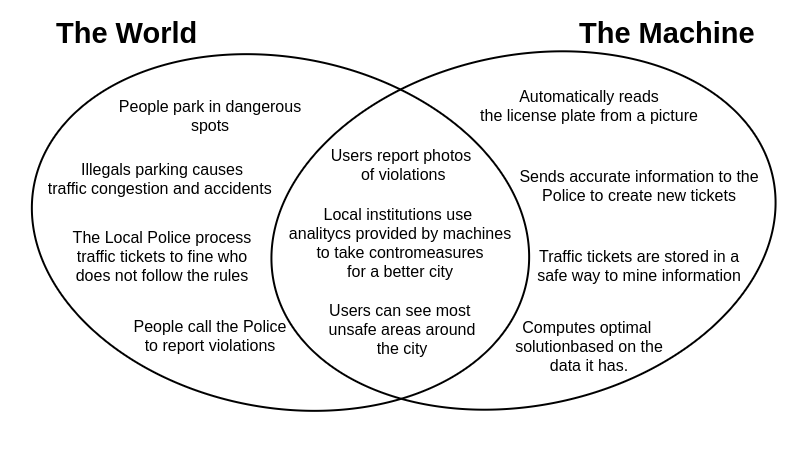
\includegraphics[scale=0.50]{images/world-machine-phenomena}
	\caption{The world-machine phenomena chart.}
	\label{fig:world-machine}
\end{figure}

	\clearpage
	\subsection{Goals}
	\begin{itemize}

\item \textbf{[\hypertarget{G1}{G1}]} Notifing officers when particular parking violations occur.

\item \textbf{[\hypertarget{G2}{G2}]} Permitting both users and officers to learn which areas have the highest frequency of violations.

\item \textbf{[\hypertarget{G3}{G3}]} Permitting both users and officers to learn which vehicles commit the most violations.

\item \textbf{[\hypertarget{G4}{G4}]} Suggesting possible interventions to potentially unsafe areas.

\item \textbf{[\hypertarget{G5}{G5}]} Allowing the local police to generate automatic traffic tickets from SafeStreets data.

\item \textbf{[\hypertarget{G6}{G6}]} Building and exhibiting statistics.

\end{itemize}
	\subsubsection{Traceability Matrix}
	Since goals, functions and constraints are related to each other a traceability matrix is provided in order to enlight the various relationships among them.
\begin{flushleft}

\begin{table}[htp]
\centering
\begin{tabular}{|l|l|l|l|}
\hline
Goal ID&Functions ID&Constraints ID&UseCases ID\\
\hline
\hyperlink{G1}{G1}&\hyperlink{sec:f1}{F1}&\hyperlink{C1}{C1}, \hyperlink{C3}{C3}, \hyperlink{C4}{C4}, \hyperlink{C6}{C6}&\hyperlink{tab:reportcreationtab}{U1}\\
\hline
\hyperlink{G2}{G2}&\hyperlink{sec:f2}{F2}&\hyperlink{C8}{C8}, \hyperlink{C3}{C3}, \hyperlink{C9}{C9}&\hyperlink{tab:dataminingtab}{U6}, \hyperlink{tab:dataminingofficertab}{U7}\\
\hline
\hyperlink{G3}{G3}&\hyperlink{sec:f3}{F3}&\hyperlink{C3}{C3}, \hyperlink{C7}{C7}, \hyperlink{C8}{C8}&\hyperlink{tab:dataminingofficertab}{U7}\\
\hline
\hyperlink{G4}{G4}&\hyperlink{sec:f4}{F4}&\hyperlink{C2}{C2}, \hyperlink{C4}{C4}, \hyperlink{C6}{C6}&\hyperlink{tab:AutomaticTrafficTicket}{U5}\\
\hline
\hyperlink{G5}{G5}&\hyperlink{sec:f2}{F2}&\hyperlink{C4}{C4}, \hyperlink{C6}{C6}, \hyperlink{C5}{C5}&\hyperlink{tab:dataminingvehicleofficerstab}{U9}, \hyperlink{tab:dataminingvehicletab}{U8}\\
\hline
\hyperlink{G6}{G6}&\hyperlink{sec:f2}{F2}, \hyperlink{sec:f5}{F5}&\hyperlink{C6}{C6}, \hyperlink{C9}{C9}&\hyperlink{tab:statisticsconsultingtab}{U10}\\
\hline
\hyperlink{G7}{G7}&-&-&\hyperlink{tab:statisticsconsultingtab}{U10}\\
\hline
-&\hyperlink{sec:f0}{F0}&-&\hyperlink{tab:signupusecase}{U1}, \hyperlink{tab:loginusecase}{U2}, \hyperlink{tab:recoverpasswordusecase}{U3}\\
\hline

\end{tabular}

\caption{Traceability Matrix} 

\end{table}

\end{flushleft}
	\subsection{Definition and Acronyms}
	\subsubsection{Definitions}
	\subsubsection{Acronyms}
	\subsection{Revision}
	\subsection{Actors}
	\begin{itemize}
	\item \textit{Guest}: This actor plays the role of a person who is not registered and thus logged in.
	\item \textit{User}: This actor refers to the condition of a normal person (not an officer) already signed up and logged.
	\item \textit{Officer} or \textit{Authority}: This actor represents a public officer that interacts with SafeStreets in some ways.
\end{itemize}
	\subsection{References}
	\begin{itemize}
	
	\item The 2019-2020 Software Engineering 2 Project Assignment document
	\item The IEEE Standard for DD
	\item The RASD of SafeStreets
	
\end{itemize}
	\subsection{Document Structure}
	\clearpage
	\section{Overall description}
	\subsection{Product perspective}
	The idea is to create an application to allow users to report parking violations without taking much time to their daily life. According to this intention, we would like to realize an extremely friendly user interface and a lightweight software in order to make SafeStreets affordable to many people as possible and runnable by many devices.\\
Users will certainly be able to exploit the advanced functions of SafeStreets such as charts and analitycs, but as those functions rely over data, the basic violations reporting function will be the core one.\\
\\
Since a small downtime of SafeStreets is not going to cause damage to anyone, it will be tolerated without much thoughts. On the other hand, as our software is going to run some kind of OCR and AI recognition algorithm that will probably be expensive in terms of resources, it should be very dynamic to support different queries in a few seconds.\\
In addition, our software is going to process very specific data that could potentially lead someone to be fined, hence it should ensure that the chain of custody is never broken and the images are never altered.\\
To upload a new picture on SafeStreets or to view charts about violations, it is obviously required an active and functional internet connection. But as said, as data are the core business of SafeStreets, there will be put in place a mechanism such that a user can insert all the information needed to report someone on his mobile application, then those information will be sent as soon as the internet connection is restored.\\
\\
Concerning the hardware, we intend to have a database which contains all the historical information about reports made by the people. This database will allow both users and officers to see both aggregated and detailed information that require an huge amount of data to be processed. Hence, the internal database engineering should take this into consideration.\\
	\subsection{Product functionalities}
	\subsection{User characteristics}
	
	\subsection{Assumptions and dependencies}
	\subsubsection{Domain Assumptions}
	\begin{enumerate}

\item A user should input only correct data when reporting a violation, for example the license plate position should be correct

\item The image and picture meta-data aren't altered by the user who first submit the report

\item The municipality will provide provide correct and complete information 
about the accidents

\item The municipality services are supposed to be functional during the uptime of SafeStreets.

\end{enumerate}
	
	\subsubsection{Domain Assumptions}
	
	\subsubsection{General Assumptions}
	
	\subsubsection{Constraints}
	
	\clearpage
\end{document}